\documentclass[12pt]{article}
\usepackage[hungarian]{babel}
\selectlanguage{hungarian}
\usepackage[utf8]{inputenc}
\usepackage[T1]{fontenc}

\pdfpageheight\paperheight
\pdfpagewidth\paperwidth
\setlength\topmargin{-1cm} \setlength\oddsidemargin{-0cm}
\setlength\textheight{25cm} \setlength\textwidth{15.8cm}
\setlength\columnsep{0.25in}  \newlength\titlebox \setlength\titlebox{2.00in}
\setlength\headheight{5pt}   \setlength\headsep{0pt}
\setlength\footskip{1cm}
\setlength\leftmargin{0.0in}

\usepackage{alltt}

\usepackage{tikz}
\usetikzlibrary{shapes,shapes.geometric,shapes.multipart,calc}
\tikzset{
  level distance=1cm, level 1/.style={sibling distance=3.5cm},
  level 2/.style={sibling distance=2.5cm},
  level 3/.style={sibling distance=1cm},
  treenode/.style = {align=center, inner sep=0pt, text centered, font=\sffamily},
  arn_n/.style = {treenode, circle, white, font=\sffamily\bfseries, draw=black, fill=black, text width=1.5em},
  arn_r/.style = {treenode, circle, white, draw=red, text width=1.5em, very thick, fill=red}
}
\usepackage{subfig}
\date{}
\title{5. gyakorlat -- Piros-fekete fa törlés}
\begin{document}

\maketitle

\noindent 1. Az alábbi piros-fekete fából töröljük a 55, 98, 30, 50, 49, 7, 73, 34 kulcsokat.

\begin{figure}[!h]
\centering
	\begin{tikzpicture}
	\node [arn_n] {54}
		child{ node [arn_n] {34}
			child{ node [arn_r] {9}
				child{ node [arn_n]  {7}
					child{ node [arn_r]  {5}}
					child[missing]
				}
				child{ node [arn_n]  {30}}
			}
			child{ node [arn_n] {50}
				child{ node [arn_r]  {49}}
				child[missing]
			}
		}
		child{ node [arn_n] {69}
			child{ node [arn_r]  {56}
				child{ node [arn_n]  {55}}
				child{ node [arn_n]  {68}}
			}
			child{ node [arn_r]  {75}
				child{ node [arn_n]  {70}
					child[missing]
					child{ node [arn_r]  {73}}
				}
				child{ node [arn_n]  {98}}			
			}
		};
	\end{tikzpicture}
\end{figure}


\begin{figure}[!h]
%\centering
\textbf{Töröl(55)}\\
\subfloat[fekete testvér+unokaöccsek $\rightarrow$ színezés]{
	\begin{tikzpicture}
	\node [arn_n] {54}
		child{ node [arn_n] {34}
			child{ node [arn_r] {9}
				child{ node [arn_n]  {7}
					child{ node [arn_r]  {5}}
					child[missing]
				}
				child{ node [arn_n]  {30}}
			}
			child{ node [arn_n] {50}
				child{ node [arn_r]  {49}}
				child[missing]
			}
		}
		child{ node [arn_n] {69}
			child{ node [arn_n]  {56}
				child[missing]
				child{ node [arn_r]  {68}}
			}
			child{ node [arn_r]  {75}
				child{ node [arn_n]  {70}
					child[missing]
					child{ node [arn_r]  {73}}
				}
				child{ node [arn_n]  {98}}
			}
		};
	\end{tikzpicture}
}\\
\textbf{Töröl (98)}\\
\subfloat[fekete testvér, piros unokaöccs $\rightarrow$ forgatás]{
	\begin{tikzpicture}
	\node [arn_n] {54}
		child{ node [arn_n] {34}
			child{ node [arn_r] {9}
				child{ node [arn_n]  {7}
					child{ node [arn_r]  {5}}
					child[missing]
				}
				child{ node [arn_n]  {30}}
			}
			child{ node [arn_n] {50}
				child{ node [arn_r]  {49}}
				child[missing]
			}
		}
		child{ node [arn_n] {69}
			child{ node [arn_n]  {56}
				child[missing]
				child{ node [arn_r]  {68}}
			}
			child{ node [arn_r]  {73}
				child{ node [arn_n]  {70}}
				child{ node [arn_n]  {75}}
			}
		};
	\end{tikzpicture}
}
\end{figure}

\begin{figure}[htb]\ContinuedFloat
%\centering
\textbf{Töröl(30)}\\
\subfloat[fekete testvér, piros unokaöccs $\rightarrow$ forgatás]{
	\begin{tikzpicture}
	\node [arn_n] {54}
		child{ node [arn_n] {34}
			child{ node [arn_r] {7}
				child{ node [arn_n]  {5}}
				child{ node [arn_n]  {9}}
			}
			child{ node [arn_n] {50}
				child{ node [arn_r]  {49}}
				child[missing]
			}
		}
		child{ node [arn_n] {69}
			child{ node [arn_n]  {56}
				child[missing]
				child{ node [arn_r]  {68}}
			}
			child{ node [arn_r]  {73}
				child{ node [arn_n]  {70}}
				child{ node [arn_n]  {75}}
			}
		};
	\end{tikzpicture}
}
\\ \textbf{Töröl(50)} \\
\subfloat[egyedüli gyereke piros $\rightarrow$ nincs teendő]{
	\begin{tikzpicture}
	\node [arn_n] {54}
		child{ node [arn_n] {34}
			child{ node [arn_r] {7}
				child{ node [arn_n]  {5}}
				child{ node [arn_n]  {9}}
			}
			child{ node [arn_n] {49}}
		}
		child{ node [arn_n] {69}
			child{ node [arn_n]  {56}
				child[missing]
				child{ node [arn_r]  {68}}
			}
			child{ node [arn_r]  {73}
				child{ node [arn_n]  {70}}
				child{ node [arn_n]  {75}}
			}
		};
	\end{tikzpicture}
}
\\ \textbf{Töröl(49)} \\
\subfloat[piros testvér $\rightarrow$ segédforgatás]{
	\begin{tikzpicture}
	\node [arn_n] {54}
		child{ node [arn_n] {7}
			child{ node [arn_n] {5}}
			child{ node [arn_r] {34}
				child{ node[arn_n] {9}}
				child{ node[arn_n]{nil}}
			}
		}
		child{ node [arn_n] {69}
			child{ node [arn_n]  {56}
				child[missing]
				child{ node [arn_r]  {68}}
			}
			child{ node [arn_r]  {73}
				child{ node [arn_n]  {70}}
				child{ node [arn_n]  {75}}
			}
		};
	\end{tikzpicture}
}~
\setcounter{subfigure}{4}
\subfloat[fekete testvér+unokaöccsek $\rightarrow$ színezés]{
	\begin{tikzpicture}
	\node [arn_n] {54}
		child{ node [arn_n] {7}
			child{ node [arn_n] {5}}
			child{ node [arn_n] {34}
				child{ node[arn_r] {9}}
				child[missing]
			}
		}
		child{ node [arn_n] {69}
			child{ node [arn_n]  {56}
				child[missing]
				child{ node [arn_r]  {68}}
			}
			child{ node [arn_r]  {73}
				child{ node [arn_n]  {70}}
				child{ node [arn_n]  {75}}
			}
		};
	\end{tikzpicture}
}
\\ \textbf{Töröl(7)} \\
\subfloat[fekete testvér+piros unokaöccs $\rightarrow$ forgatás]{
	\begin{tikzpicture}
	\node [arn_n] {54}
		child{ node [arn_n] {9}
			child{ node [arn_n] {5}}
			child{ node [arn_n] {34}}
		}
		child{ node [arn_n] {69}
			child{ node [arn_n]  {56}
				child[missing]
				child{ node [arn_r]  {68}}
			}
			child{ node [arn_r]  {73}
				child{ node [arn_n]  {70}}
				child{ node [arn_n]  {75}}
			}
		};
	\end{tikzpicture}
}
\\ \textbf{Töröl(73)}  \hfil \textbf{Töröl(34)}\\
\subfloat[fekete testvér+unokaöccsek $\rightarrow$ átszínezés]{
	\begin{tikzpicture}
	\node [arn_n] {54}
		child{ node [arn_n] {9}
			child{ node [arn_n] {5}}
			child{ node [arn_n] {34}}
		}
		child{ node [arn_n] {69}
			child{ node [arn_n]  {56}
				child[missing]
				child{ node [arn_r]  {68}}
			}
			child{ node [arn_n]  {70}
				child[missing]
				child{ node [arn_r]  {75}}
			}
		};
	\end{tikzpicture}
}~
%\end{figure}
%\begin{figure}[!ht]\ContinuedFloat
%\centering
\subfloat[fekete testvér+unokaöccsek $\rightarrow$ átszínezés]{
	\begin{tikzpicture}
	\node [arn_n] {54}
		child{ node [arn_n] {9}
			child{ node [arn_r] {5}}
			child[missing]
		}
		child{ node [arn_r] {69}
			child{ node [arn_n]  {56}
				child[missing]
				child{ node [arn_r]  {68}}
			}
			child{ node [arn_n]  {70}
				child[missing]
				child{ node [arn_r]  {75}}
			}
		};
	\end{tikzpicture}
}
\end{figure}

\clearpage

\noindent 2. Adjuk meg az előző feladat kezdeti piros-fekete fájával ekvivalens 2-3-4 fát!
	\begin{figure}[!ht]
		\centering
		\begin{tikzpicture}
			\tikzstyle{bnode}=[rectangle split, rectangle split parts=3, rectangle split horizontal,rectangle split ignore empty parts,draw, fill=white]
			\tikzstyle{every node}=[bnode]
			\tikzstyle{level 1}=[sibling distance=7cm]
			\node {54}
				child {node{\color{red}{9} \nodepart{two} 34}
					child[sibling distance=2cm]{node{\color{red}{5} \nodepart{two} 7}}
					child[sibling distance=2cm]{node{30}}
					child[sibling distance=2cm]{node{\color{red}{49} \nodepart{two} 50}}
				}
				child {node{\color{red}{56} \nodepart{two} 69 \nodepart{three} \color{red}{75}}
					child[sibling distance=2cm]{node{55}}
					child[sibling distance=2cm]{node{68}}
					child[sibling distance=2cm]{node{70 \nodepart{two} \color{red}{73}}}
					child[sibling distance=2cm]{node{98}}
				};
		\end{tikzpicture}
	\end{figure}
	
	Megoldás: az eredeti fa fekete színű csúcsait ''olvasszuk össze'' piros színű gyerekeikkel.
	
	Mi lenne a törlések végrehajtását követően előálló 2-3-4 fa?

	\begin{figure}[!ht]
		\centering
		\begin{tikzpicture}
			\tikzstyle{bnode}=[rectangle split, rectangle split parts=3, rectangle split horizontal,rectangle split ignore empty parts,draw, fill=white]
			\tikzstyle{every node}=[bnode]
			\node {54 \nodepart{two} \color{red}{69}}
				child {node{\color{red}{5} \nodepart{two} 9}}
				child {node{58 \nodepart{two} \color{red}{68}}}
				child {node{70 \nodepart{two} \color{red}{75}}
			};
		\end{tikzpicture}
	\end{figure}

\end{document}